Dans ce chapitre, nous allons passer en revue les différentes décisions techniques qui ont été prises ainsi que les outils utilisés, et présenter les résultats obtenus.

\section{Choix techniques et motivations}\label{sec: conception-choix-techniques-et-motivation}
\subsection*{MySQL}\label{subsec:conception-mysql}
Le choix de la base de données est une étape cruciale dans le développement d'une application. Il existe plusieurs types de bases de données, chacune ayant ses avantages et inconvénients propres.

Dans le cadre de ce projet, nous avons opté pour une base de données relationnelle, car elle s'adapte le mieux à notre cas d'utilisation. Elle nous permet de stocker les données de manière structurée et de les manipuler aisément à l'aide de requêtes SQL.

Nous avons choisi d'utiliser MySQL, une base de données relationnelle populaire dotée d'une large communauté de développeurs et d'une documentation exhaustive


\subsection*{Architecture de l'application}\label{subsec: conception-application-architecture}
Notre application repose sur une architecture client-serveur. Le serveur assure la gestion des données et la logique métier, tandis que le client gère l'interface utilisateur. Pour communiquer avec le serveur, le client utilise une API REST (Representational State Transfer), qui repose sur un ensemble de conventions et de bonnes pratiques pour la conception d'API web.

Cette API REST permet au client d'effectuer des opérations CRUD (Create, Read, Update, Delete) sur les données stockées sur le serveur. Nous avons choisi d'utiliser une API REST pour sa simplicité de mise en œuvre et son utilisation aisée. Elle permet également de séparer la logique métier de l'interface utilisateur, facilitant ainsi la maintenance et l'évolutivité de l'application.

Nous utilisons le format de données JSON (JavaScript Object Notation) pour l'API REST, car il est léger, facile à lire et à écrire.
\subsection*{Le processus unifié}\label{subsec: conception-unified-process}
Nous avons choisi d'utiliser le processus unifié pour le développement de
notre application. Le processus unifié est un processus de développement de
logiciels itératif et incrémental de la famille des méthodes agiles.

le processus unifié utilise des modèles UML (Unified Modeling Language) pour la
conception et la modélisation.

\subsection*{Typescript}\label{subsec: conception-typescript}
Nous avons choisi d'utiliser le langage de programmation Typescript pour le développement de notre application. Typescript est un langage open source développé par Microsoft, conçu pour le développement d'applications JavaScript à grande échelle. Il ajoute des fonctionnalités au JavaScript, comme le typage statique, les classes, les interfaces, les modules, etc. Il est compilé en JavaScript, ce qui permet son utilisation sur n'importe quel navigateur web ou serveur web.

Le principal avantage de Typescript est qu'il est facile à apprendre et à utiliser. Il permet de détecter les erreurs de programmation avant l'exécution du code, ce qui facilite le débogage et améliore la qualité du code. De plus, étant compilé en JavaScript, il permet d'avoir un code client et serveur en Typescript, ce qui évite de changer de langage entre le client et le serveur.
\subsection*{NestJS}\label{subsec: conception-nestjs}
Pour le développement de la partie serveur de notre API, nous avons choisi d'utiliser
le framework open source NestJS. Ce framework est spécialement conçu pour
le développement d'applications Node.js, basé sur Express et utilisant Typescript.

Il permet de créer des applications évolutives et efficaces grâce à son architecture
modulaire. NestJS est composé de plusieurs modules, chacun ayant sa propre fonctionnalité.

\subsection*{ReactJs}\label{subsec: conception-nextjs}
Nous avons choisi d'utiliser ReactJs pour le développement de notre interface utilisateur (partie client).
web. ReactJs est une bibliothèque JavaScript open source pour la création
d'interfaces utilisateur. Il est conçu pour faciliter la création d'interfaces
utilisateur interactives et réutilisables. Il est utilisé par de nombreuses
entreprises, dont Facebook, Instagram, Netflix, Airbnb, etc.

\subsection*{Git}\label{subsec: conception-git}
Nous avons adopté Git pour la gestion de version de notre code. Git est un système de contrôle de version distribué open source, conçu pour gérer efficacement les petits et grands projets. Il permet de suivre les modifications apportées au code source et facilite la collaboration entre les développeurs.

Nous avons choisi Git pour sa facilité d'apprentissage et d'utilisation. Il nous permet de suivre les modifications apportées au code source et de revenir à une version antérieure du code si nécessaire.

\subsection*{GitHub}\label{subsec: conception-github}
Nous avons décidé d'héberger notre code sur GitHub. GitHub est un service d'hébergement de code source basé sur Git, conçu pour faciliter la collaboration entre les développeurs. Il permet d'héberger des projets open source et privés.

Nous avons choisi GitHub pour son accessibilité et sa facilité d'utilisation. Étant donné que notre projet est open source, nous souhaitons offrir la possibilité à ceux qui le souhaitent de contribuer facilement au projet.

\subsection*{Tailwindcss}\label{subsec: conception-tailwind}
Pour le développement de notre interface utilisateur côté client, nous avons opté pour le framework css Tailwindcss. Ce framework adopte l'approche utility-first, qui consiste à privilégier l'utilisation de classes utilitaires pour définir les styles plutôt que de créer des classes spécifiques à chaque élément.

Tailwindcss permet de créer des interfaces utilisateur de manière rapide et efficace, grâce à sa bibliothèque de classes utilitaires prédéfinies

\subsection*{Conclusion}\label{subsec: conception-conclusion-choix-techniques}
Nous sommes conscients que toutes les décisions prises ne sont pas forcément les meilleures, mais elles ont été prises en fonction des contraintes et des objectifs du projet.

Notre objectif est de résoudre le problème de la délibération tout en fournissant une solution facile à maintenir et à faire évoluer à l'avenir, et également facilement adaptable à d'autres problèmes similaires, avec une grande extensibilité.

Le choix d'une API offre une grande flexibilité et une grande extensibilité, car la solution peut être utilisée par d'autres applications et facilement intégrée à d'autres systèmes. Elle peut également être utilisée pour concevoir d'autres types d'applications, tels que des applications mobiles, web ou desktop.
\section{Présentation des résultats}
\subsection{Présentation de l'API Rest}\label{sec:presentation-de-l-api}
Notre API comprend un total de 44 routes que nous avons catégorisées en 9 groupes, en fonction de la ressource qu'elles manipulent ou de leur tâche respective

\subsubsection*{Les routes de l'authentification}\label{subsec:routes-auth}

\begin{table}[ht]
  \centering
  \caption{Tableau des routes de l'authentification}
  \label{tab:routes-auth}
  \begin{tabular}{|p{2.5cm}|p{1cm}|p{3.5cm}|p{4cm}|}
    \hline
    Méthode  & Params & Corps & Réponses \\
    \hline
        POST   /login & - & \{ email, mot de passe \}  & \{ jeton \} \\
    \hline
        GET  /profile & - & - &  utilisateur: \{ id, nom, email, mot de passe, est\_actif \}  \\
    \hline
        PATCH /profile & - & \{ nom, email \} & \{ status, message \} \\
    \hline
        PATCH /update-password & - & \{ Ancien mot de passe, nouveau mot de passe \} & \{ status, message \} \\
    \hline
  \end{tabular}
\end{table}
\pagebreak

\subsubsection*{Les routes de la gestion des facultés}\label{subsec:routes-fac}

\begin{table}[ht]
  \caption{Tableau des routes de la gestion des facultés}
  \label{tab:routes-fac}
  \begin{tabular}{|p{1.5cm}|p{1.5cm}|p{1.5cm}|p{1.5cm}|p{4cm}|}
    \hline
          Méthode & Action & Params & Corps & Réponse \\
      \hline
          POST /  & Créer &  - & \{ nom \} & \{ status, message \} \\
      \hline
          GET  / & Lire  & - & - & facultés[] : \{ id, nom \}  \\
      \hline
          GET /:id  & Lire  & \{ id \} & - & facultés : \{ id, nom \}  \\
      \hline
          PATCH  /:id  & Modifier & \{ id \} & \{ nom \} & \{ status, message \} \\
      \hline
          DELETE  /:id  & Supprimer & \{ id \} & - & \{ status, message \} \\
      \hline
  \end{tabular}
\end{table}
\pagebreak

\subsubsection*{Les routes de la gestion des filières}\label{subsec:routes-field}

\begin{table}[ht]
  \caption{Tableau des routes de la gestion des filières}
  \label{tab:routes-field}
  \begin{tabular}{|p{1.5cm}|p{1.5cm}|p{1.5cm}|p{2.5cm}|p{3cm}|}
    \hline
      Méthode & Action & Params & Corps & Réponse \\
    \hline
        POST / & Créer &  - & \{ nom, faculté \} & \{ status, message \} \\
    \hline
        GET / & Lire & - & - & filières[] : \{ id, nom, faculté \}  \\
    \hline
        GET /:id & Lire & \{ id \} & - & filière: \{ id, nom, faculté \} \\
    \hline
        PATCH /:id & Modifier & \{ id \} & \{ nom, faculté \} & \{ status, message \} \\
    \hline
        DELETE /:id & Supprimer & \{ id \} & - & \{ status, message \} \\
    \hline
  \end{tabular}
\end{table}
\pagebreak

\subsubsection*{Les routes de la gestion des cours}\label{subsec:routes-course}

\begin{table}[ht]
  \caption{Tableau des routes de la gestion des cours}
  \label{tab:routes-course}
  \begin{tabular}{|p{1.5cm}|p{1.5cm}|p{1.5cm}|p{2.5cm}|p{3.5cm}|}
    \hline
      Méthode & Action & Params & Corps & Réponse \\
    \hline
      POST / & Créer &  - &  \{ nom, heures, crédits, promotion, enseignant, filière \} & \{ status, message \} \\
    \hline
        GET /  & Lire & - & - & cours[] :  \{ id, nom, heures, crédits, promotion, enseignant, filière \} \\
    \hline
        GET /:id & Lire & \{ id \} & - & cours: \{ id, nom, heures, crédits, promotion, enseignant, filière \} \\
    \hline
        PATCH /:id & Modifier  & \{ id \} &  \{ nom, heures, crédits, promotion, enseignant, filière \} & \{ status, message \} \\
    \hline
        DELETE /:id & Supprimer & \{ id \} & - & \{ status, message \} \\
    \hline
  \end{tabular}
\end{table}
\pagebreak

\subsubsection*{Les routes de la gestion des étudiants}\label{subsec:routes-student}

\begin{table}[ht]
  \caption{Tableau des routes de la gestion des étudiants}
  \label{tab:routes-student}
  \begin{tabular}{|p{1.5cm}|p{1cm}|p{1.5cm}|p{3cm}|p{3.5cm}| }
    \hline
    Méthode & Route & Paramètre & Corps & Réponses \\
    \hline
    GET & / & - & - & \{ étudiants[] \} \\
    \hline
    GET & /:id & \{ id \} & - & étudiant : \{ id, nom, matricule, email, filière, cours[] \} \\
    \hline
    POST & / & - & \{ nom, matricule, email, filière \} & \{ status, message \} \\
    \hline
    PATCH & /:id & \{ id \} & \{ nom, matricule, email, filière \} & \{ status, message \} \\
    \hline
    DELETE & /:id & \{ id \} & - & \{ status, message \} \\
    \hline
    GET fields/:fieldId/promotions/promotionId & Lire & \{ fieldId, promotionId \} & - &  étudiants[] : \{ id, nom, email, matricule, filière, promotion \} \\
    \hline
    GET courses/:coursID & Lire & \{ coursId \} & - &  étudiants[] : \{ id, nom, email, matricule, promotion, compléments \} \\
    \hline
  \end{tabular}
\end{table}
\pagebreak

\subsubsection*{Les routes de la gestion des cotes}\label{subsec:routes-grade}

\begin{table}[ht]
  \caption{Tableau des routes de la gestion des cotes}
  \label{tab:routes-grade}
  \begin{tabular}{|p{1.5cm}|p{1cm}|p{1cm}|p{3cm}|p{4cm}| }
    \hline
    Méthode & Route & Params & Corps & Réponses \\
    \hline
        POST /  & Créer &  - &\{ moyenne, moyenne\_eg, session, promotion\_etudiant, cours, étudiant \} & \{ status, message \} \\
    \hline
        GET  / & Lire & - & - & cotes[] :  \{ id, moyenne, moyenne\_eg, session, promotion\_etudiant, cours, étudiant \} \\
    \hline
        GET  /:id  & Lire & \{ id \} & - & cote: \{id, moyenne, moyenne\_eg, session, promotion\_etudiant, cours, étudiant \} \\
    \hline
        PATCH /:id  & Modifier & \{ id \} & \{ id, moyenne, moyenne\_eg, session, promotion\_etudiant, cours, étudiant \} & \{ status, message \} \\
    \hline
        DELETE  /:id & Supprimer  & \{ id \} & - & \{ status, message \} \\
    \hline
  \end{tabular}
\end{table}
\pagebreak

\subsubsection*{Les routes de la gestion des délibérations}\label{subsec:routes-deliberation}

\begin{table}[ht]
  \caption{Tableau des routes de la gestion des délibérations}
  \label{tab:routes-deliberation}
  \begin{tabular}{|p{2cm}|p{1cm}|p{1cm}|p{1.5cm}|p{4cm}| }
    \hline
    Méthode & Route & Params & Corps & Réponses \\
    \hline
    GET /:id & Lire &  \{ id \} & - & \{ nom, matricule, email, filière, cours[] \} \\
    \hline
    GET generate-reports/:id  & Lire &  \{ id \} & - & \{ status, message \} \\
    \hline
    GET send-reports/:id & Lire &  \{ id \} & - & \{ status, message \} \\
    \hline
  \end{tabular}
\end{table}
\pagebreak

\subsubsection*{Les routes de la gestion des utilisateurs}\label{subsec:routes-user}

\begin{table}[ht]
  \caption{Tableau des routes de la gestion des utilisateurs}
  \label{tab:routes-user}
  \begin{tabular}{|p{1.5cm}|p{1.5cm}|p{1cm}|p{2.5cm}|p{3.5cm}| }
    \hline
    Méthode & Route & Params & Corps & Réponses \\
    \hline
    GET / & Lire & - & - & utilisateurs[] :  \{ id, nom, email, mot de passe, est\_actif, r\^oles[] \} \\
    \hline
    GET /:id & Lire & \{ id \} & - & utilisateur : \{ id, nom, email, mot de passe, est\_actif, r\^oles[] \} \\
    \hline
    POST / & Créer & - & \{ nom, email, r\^oles[] \} & \{ status, message \} \\
    \hline
    PATCH /:id & Modifier & \{ id \} & \{ nom, email, r\^oles[] \} & \{ status, message \} \\
    \hline
    DELETE /:id & Supprimer & \{ id \} & - & \{ status, message \} \\
    \hline
  \end{tabular}
\end{table}
\pagebreak

\subsubsection*{Les routes de la gestion des rôles}\label{subsec:routes-role}

\begin{table}[ht]
  \caption{Tableau des routes de la gestion des rôles}
  \label{tab:routes-role}
  \begin{tabular}{|p{1.5cm}|p{1.5cm}|p{1cm}|p{2.5cm}|p{3.5cm}| }
    \hline
    Méthode & Route & Params & Corps & Réponses \\
    \hline
    GET / & Lire & - & - & rôles[] :  \{ id, nom \} \\
    \hline
    GET /:id & Lire & \{ id \} & - & rôle : \{ id, nom \} \\
    \hline
    POST / & Créer & - & \{ nom \} & \{ status, message \} \\
    \hline
    PATCH /:id & Modifier & \{ id \} & \{ nom \} & \{ status, message \} \\
    \hline
    DELETE /:id & Supprimer & \{ id \} & - & \{ status, message \} \\
    \hline
  \end{tabular}
\end{table}

\subsection{Présentation de l'interface utilisateur}\label{sec:presentation-de-l-interface-utilisateur}

\subsubsection*{Authentification}\label{subsec:authentification}
L'authentification est la première étape de l'utilisation de l'application. Elle permet à l'utilisateur de s'identifier et d'accéder à l'application. L'authentification est gérée par le serveur, qui vérifie les informations d'identification de l'utilisateur et lui renvoie un jeton d'authentification s'il est valide.

\begin{figure}[ht]
  \centering
  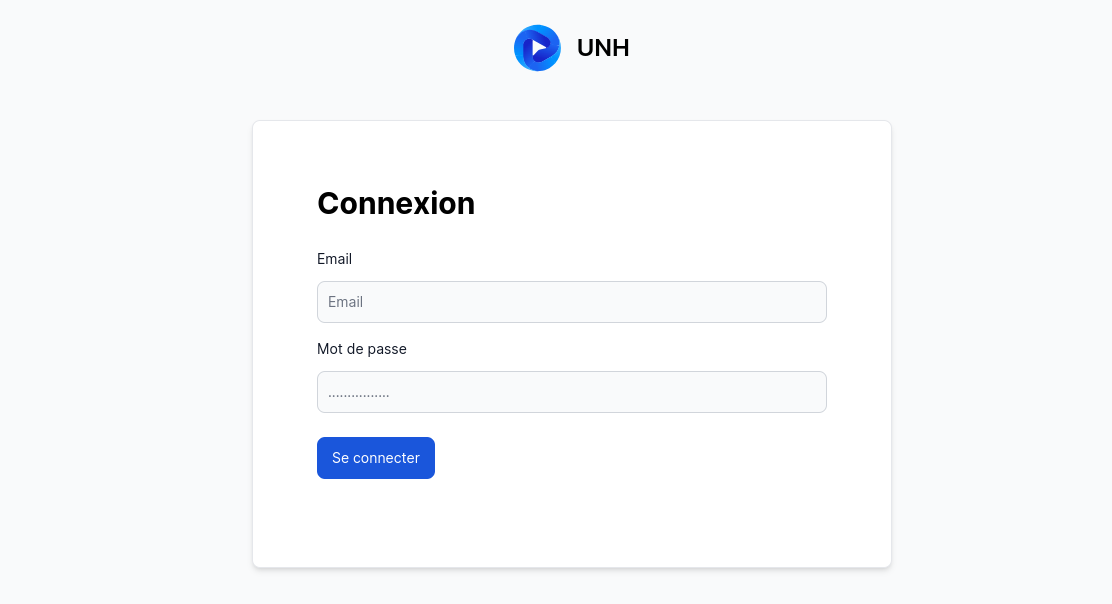
\includegraphics[width=0.8\textwidth]{gfx/ui/login}
  \caption{Page d'authentification}
  \label{fig:login}
\end{figure}


\subsubsection*{Tableau de bord}\label{subsec:tableau-de-bord}
Le tableau de bord est la page d'accueil de l'application. Il permet à l'utilisateur de voir les statistiques de l'application, telles que le nombre d'étudiants, de cours, de promotions, etc. Il permet également à l'utilisateur de naviguer vers les différentes pages de l'application.

\begin{figure}[ht]
  \centering
  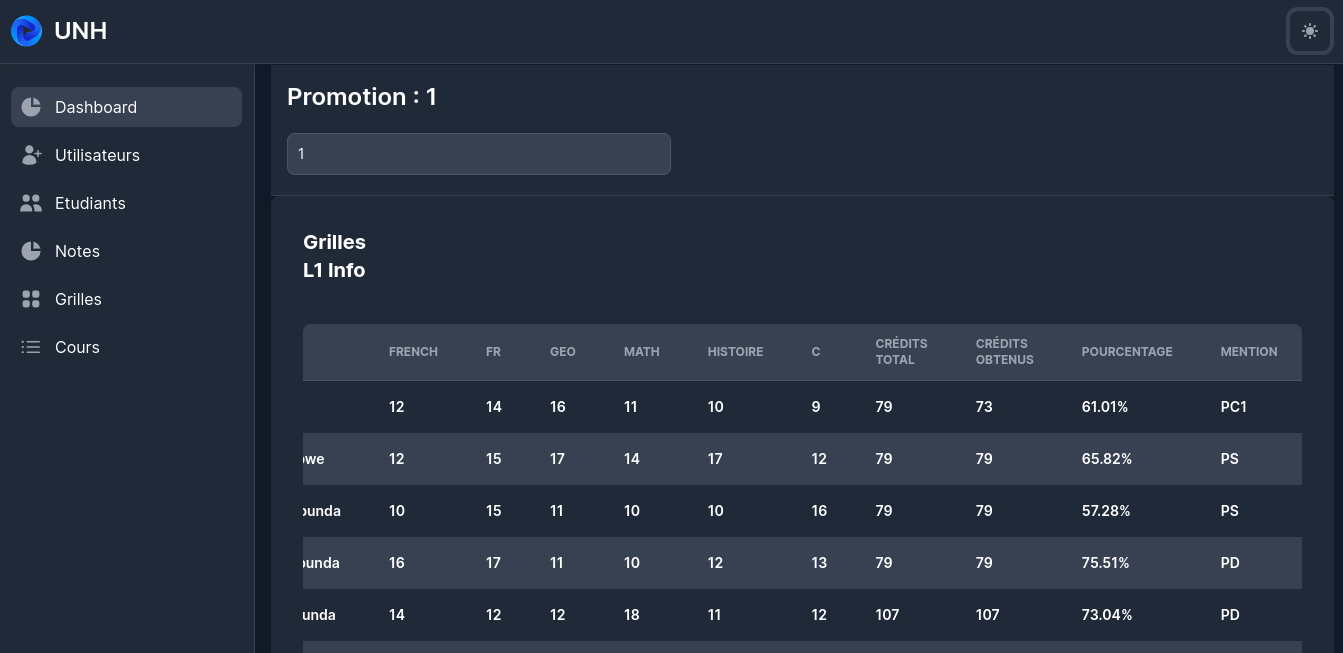
\includegraphics[width=0.8\textwidth]{gfx/ui/grid}
  \caption{Tableau de bord}
  \label{fig:dashboard}
\end{figure}

\subsubsection*{Utilisateurs}\label{subsec:utilisateurs}
La page des utilisateurs permet à l'utilisateur de gérer les utilisateurs de l'application. Il peut créer, modifier et supprimer des utilisateurs. Il peut également modifier les rôles des utilisateurs.

\begin{figure}[ht]
  \centering
  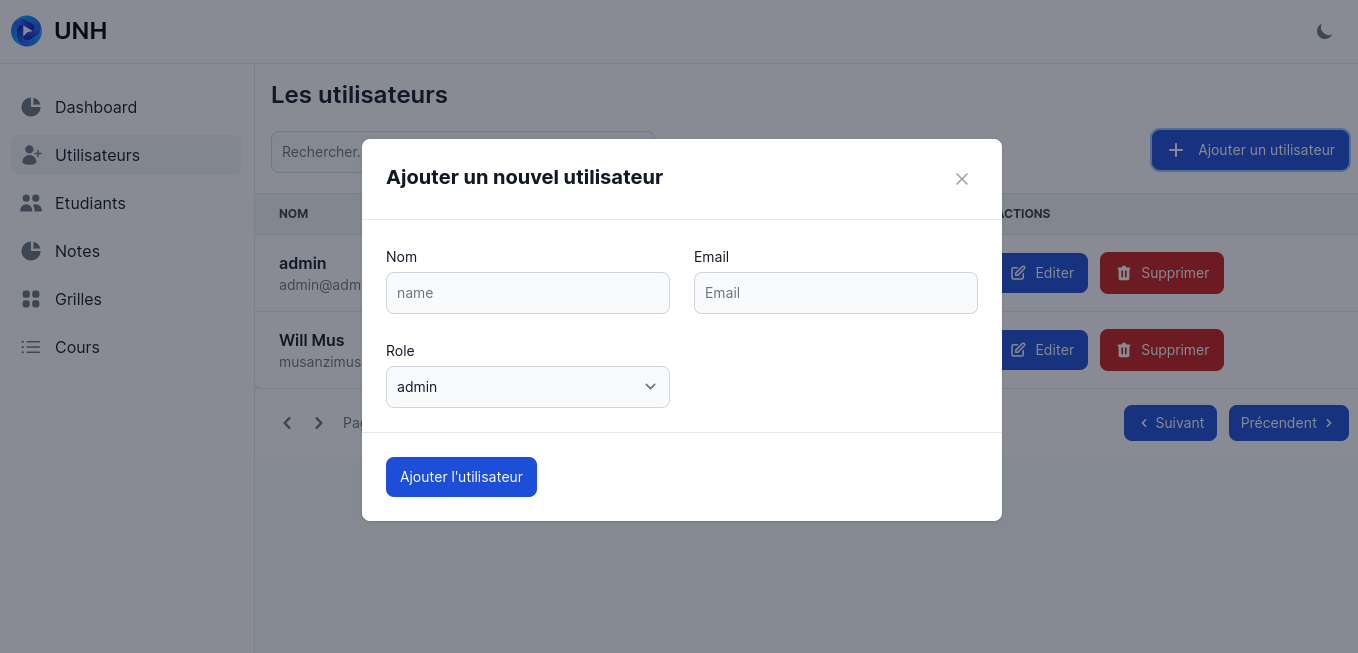
\includegraphics[width=0.8\textwidth]{gfx/ui/users}
  \caption{Page des utilisateurs}
  \label{fig:users}
\end{figure}

\subsubsection*{Cotes}\label{subsec:cotes}
La page des cotes permet à l'utilisateur de gérer les cotes des étudiants. Il peut créer, modifier et supprimer des cotes.

\begin{figure}[ht]
  \centering
  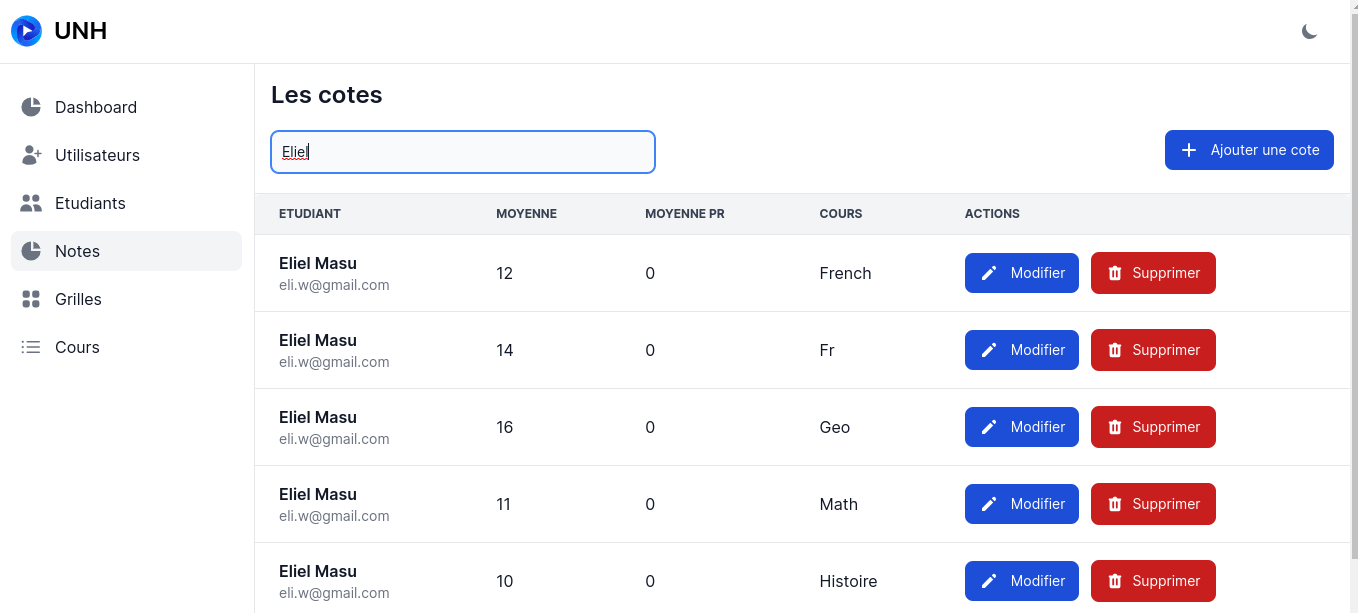
\includegraphics[width=0.8\textwidth]{gfx/ui/grades-filter}
  \caption{Page des cotes}
  \label{fig:grades}
\end{figure}

\subsubsection*{Relvés}\label{subsec:releves}
La page des relevés permet à l'utilisateur de générer et d'envoyer des relevés aux étudiants.

\begin{figure}[ht]
  \centering
  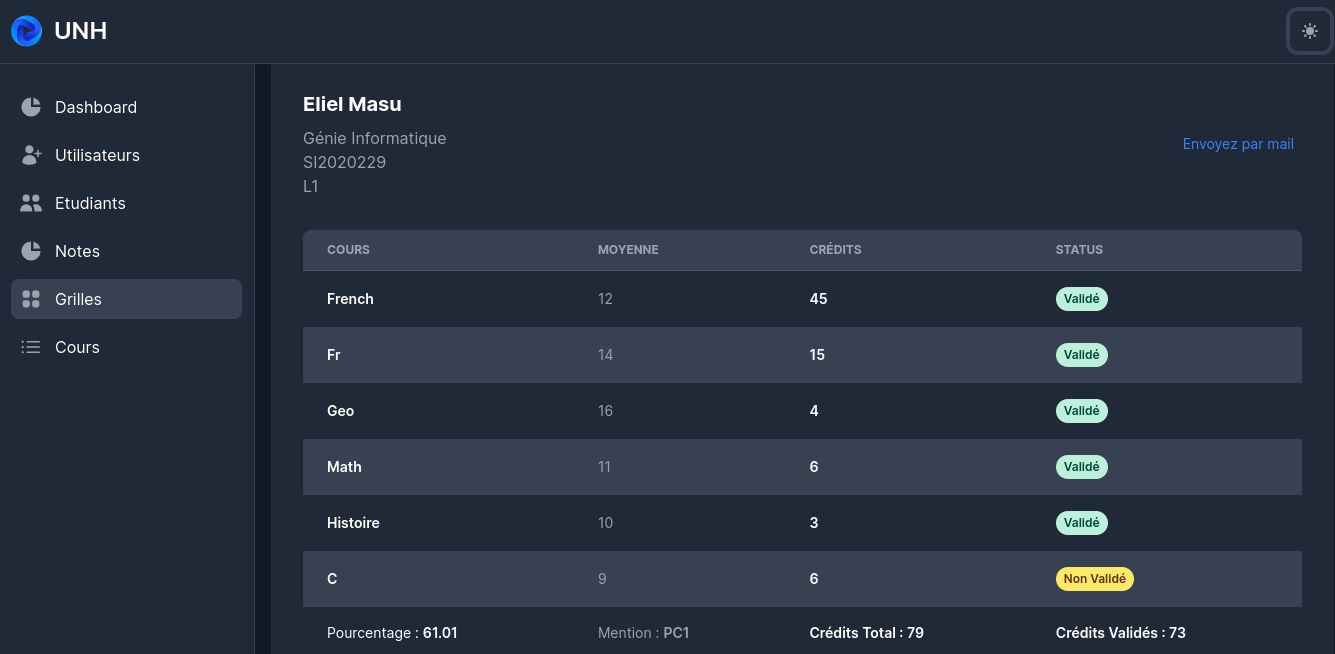
\includegraphics[width=0.8\textwidth]{gfx/ui/personnal-grid}
  \caption{Page des relevés}
  \label{fig:reports}
\end{figure}

